
% ==================================================
%	Durchführung
% ==================================================

\section{Aufbau und Durchführung}

Um die Kristallstruktur eines Probenmaterials zu bestimmen, wird die Probe mit
monochromatischen Röntgenlicht bestrahlt und die Beugungswinkel der
entstehenden Bragg-Reflexe ausgemessen.
In der Auswertung ist es schließlich die Aufgabe die, den Beugungswinkeln
entsprechenden Netzebenen, zu finden. Dabei ist es sinnvoll die Netzebenen zu
identifizieren, bei denen kein gebeugter Strahl erzeugt wird, da hierfür gerade
der Strukturfaktor verschwindet. Anhand dieser Reflexe, lässt sich in vielen
Fällen die Kristallstruktur bestimmen.

\begin{figure}[htpb]
  \centering
  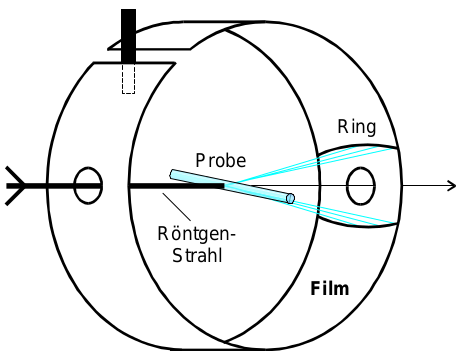
\includegraphics[scale=0.5]{bilder/aufbau.png}
  \caption{Schematische Darstellung des Versuchsaufbaus.}
\label{fig:aufbau}
\end{figure}

Im Allgemeinen ist es schwierig Bragg-Reflexe zu erzeugen, weshalb in diesem
Versuch das Debye-Scherrer-Verfahren verwandt wird, in dem kein Einkristall
sondern eine fein pulverisierte Probe benutzt wird.
In dieser Probe sind die Mikrokristalle statistisch über den Raum verteilt,
sodass es sehr wahrscheinlich ist, bei jeder Einstrahlrichtung einen
Reflexstellung eines Kristalliten zu finden.
Der Nachweis der gebeugten Röntgenstrahlung geschieht hier mit Hilfe eines
Filmstreifens.
Der schematische Aufbau des Versuchs ist in Abbildung~\ref{fig:aufbau} gezeigt.
Das Röntgenlicht der Quelle tritt hier durch eine kleine Öffnung in ein
zylindrisches Gehäuse ein, in dessen Mitte sich die Probe, ein auf einem
Glasröhrchen aufgetragenes Probenmaterial, befindet.
Das an der Probe reflektierte Röntgenlicht trifft nun auf die Gehäusewand, an
welcher der Filmstreifen befestigt ist. Die dabei unter einem Winkel $\vartheta$
gebeugte Strahlung wird sich aufgrund der statistischen Verteilung der
Kristalliten auf einem Kegelwinkel mit Öffnungswinkel $2\vartheta$ befinden.
So werden nahezu kreisförmige Linien auf dem Filmstreifen erhalten.

Hierbei können nun noch zwei zu beachtenden systematischen Fehler auftreten.
\begin{enumerate}
  \item Die Probenachse fällt nicht mit der Achse des Filmzylinders zusammen.
    Dadurch werden die Ringe um einen systematischen Fehler vergrößert oder
    verkleinert. Die Korrektur $\Delta a_V$ zu Gitterkonstanten  $a$ beträgt
    hierbei
    \begin{equation}
      \frac{\Delta a_V}{a} = \frac{v}{\cos^2\vartheta}~,
      \label{eq:a_V}
    \end{equation}
    wobei $v$ die Verschiebung der Symmetrieachsen und $R$ der Radius des
    Filmzylinders ist.
  \item Die Probe absorbiert die einfallende Röntgenstrahlen nahezu
    vollständig. Dadurch findet die Beugung nur an einem schmalen Streifen der
    Probe statt, wodurch der Winkel $\vartheta$ systematisch zu groß gemessen
    wird. Die Korrektur lautet hierbei
    \begin{equation}
      \frac{\Delta a_A}{a} = \frac{\rho}{2R}
      \qty(1 - \frac{R}{F})\frac{\cos^2\vartheta}{\vartheta}~,
      \label{eq:a_A}
    \end{equation}
    wobei $\rho$ der Radius der Probe und $F$ der Abstand Fokus-Probe ist.
\end{enumerate}

